\begin{Large}
\begin{frame}[plain]
\frametitle{Switch Data Planes today}
Two key decisions on a per-packet basis:
\begin{itemize}
\item[]
\item Scheduling: Which packet to transmit next?
\item[]
\item Queue Management: How long can queues grow? Which packet to drop?
\end{itemize}
\end{frame}

\begin{frame}[plain]
\frametitle{The long lineage of in-network algorithms}
%\only<1>{\noindent \hspace{-.75 cm} \includegraphics[width=1.0\textwidth]{march-5.pdf}}
\only<1>{\noindent \hspace{-.75 cm} 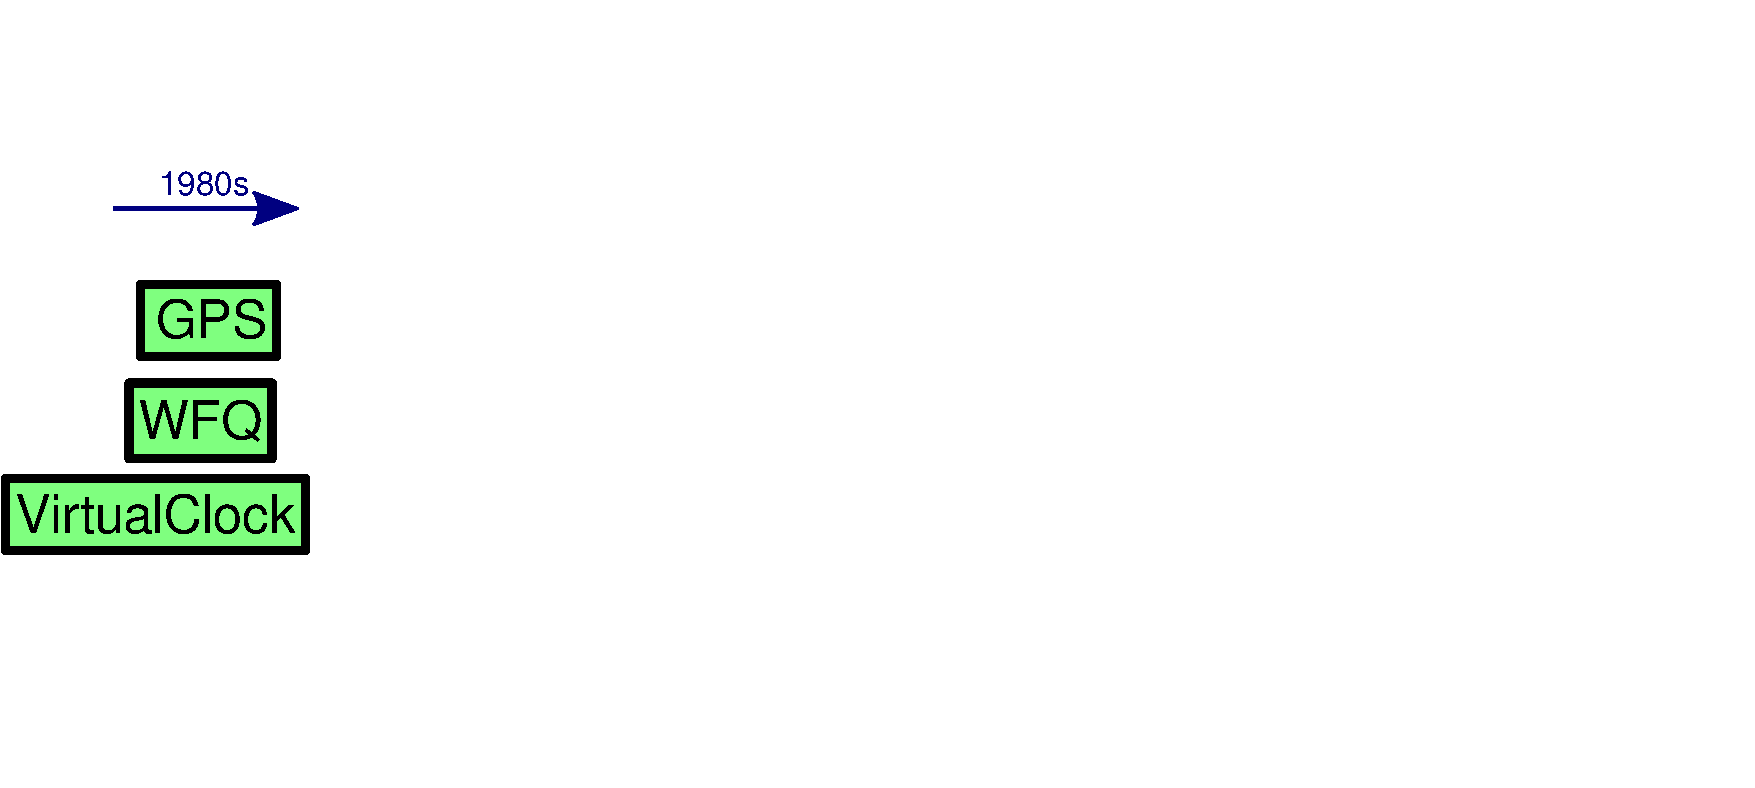
\includegraphics[width=1.0\textwidth]{march-4.pdf}}
\only<2>{\noindent \hspace{-.75 cm} 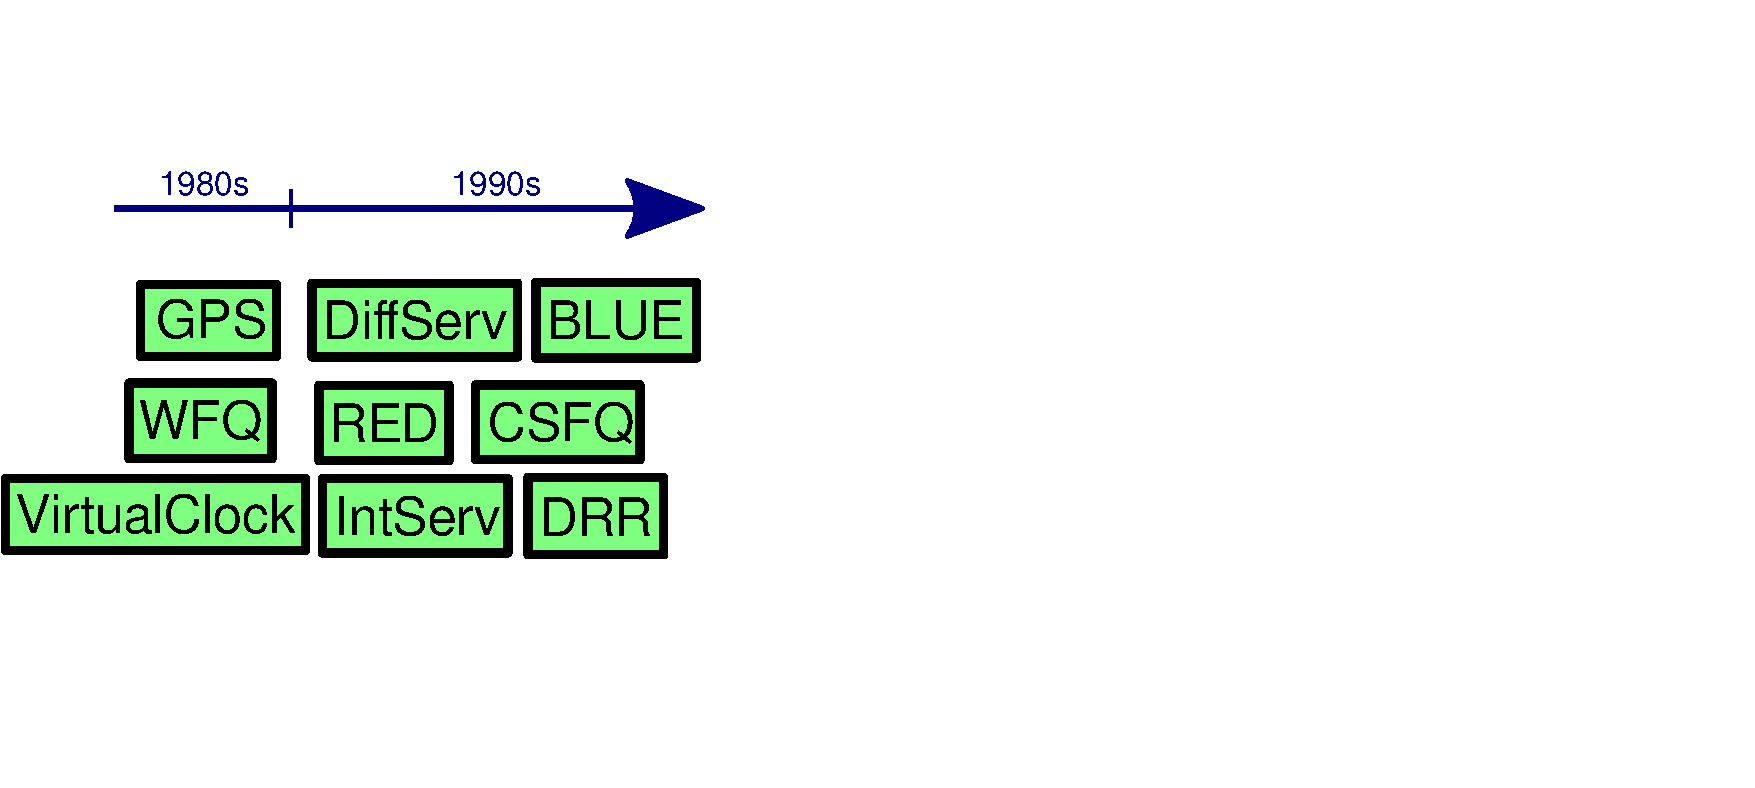
\includegraphics[width=1.0\textwidth]{march-3.pdf}}
\only<3>{\noindent \hspace{-.75 cm} 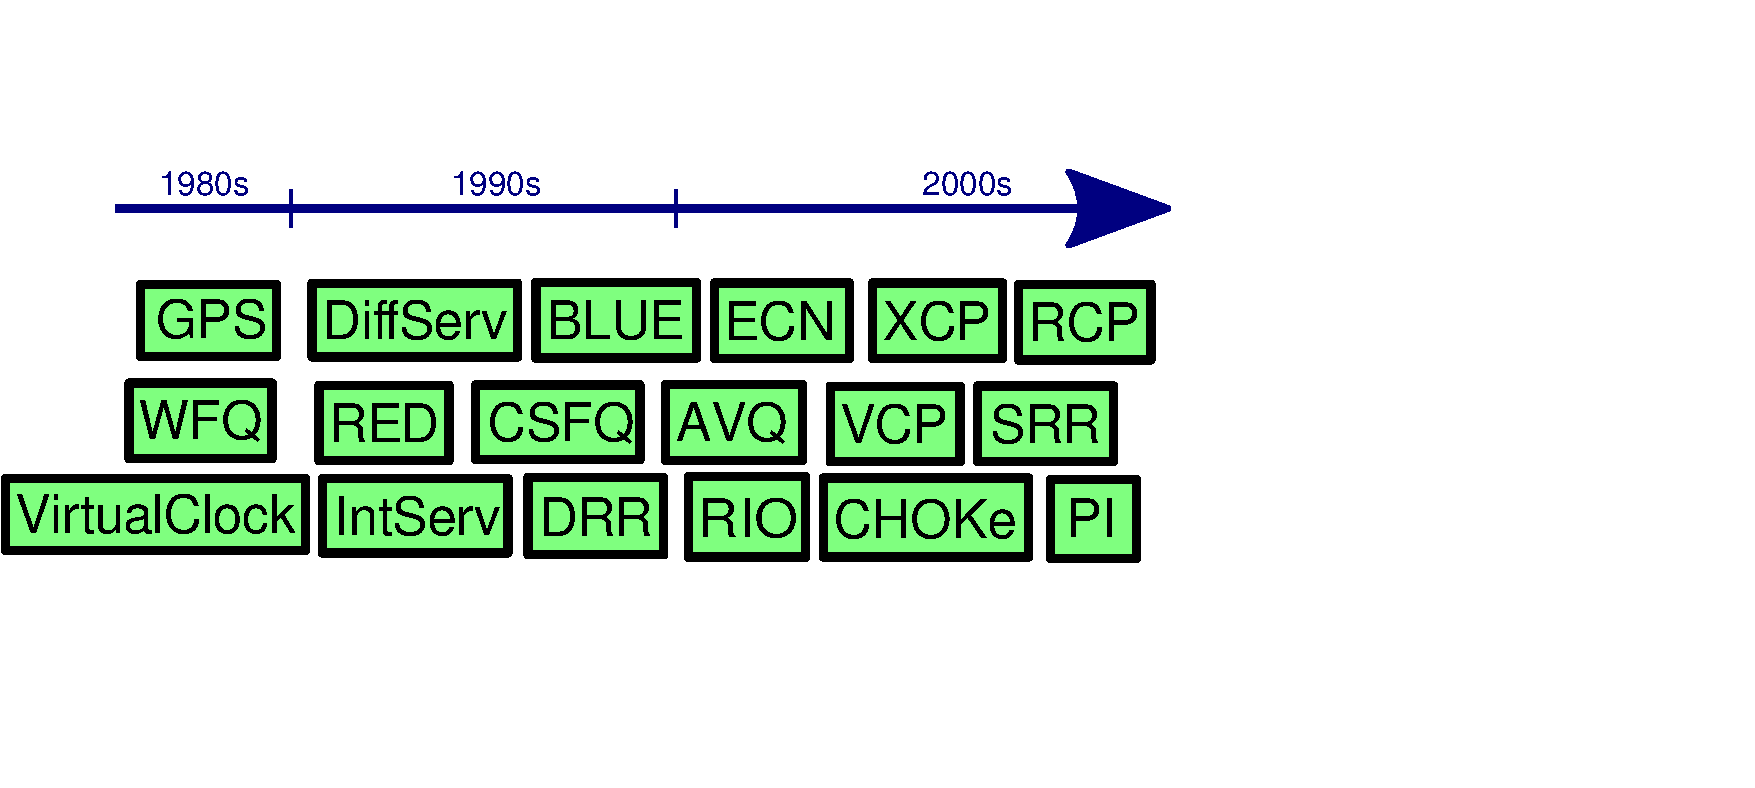
\includegraphics[width=1.0\textwidth]{march-2.pdf}}
\only<4>{\noindent \hspace{-.75 cm} 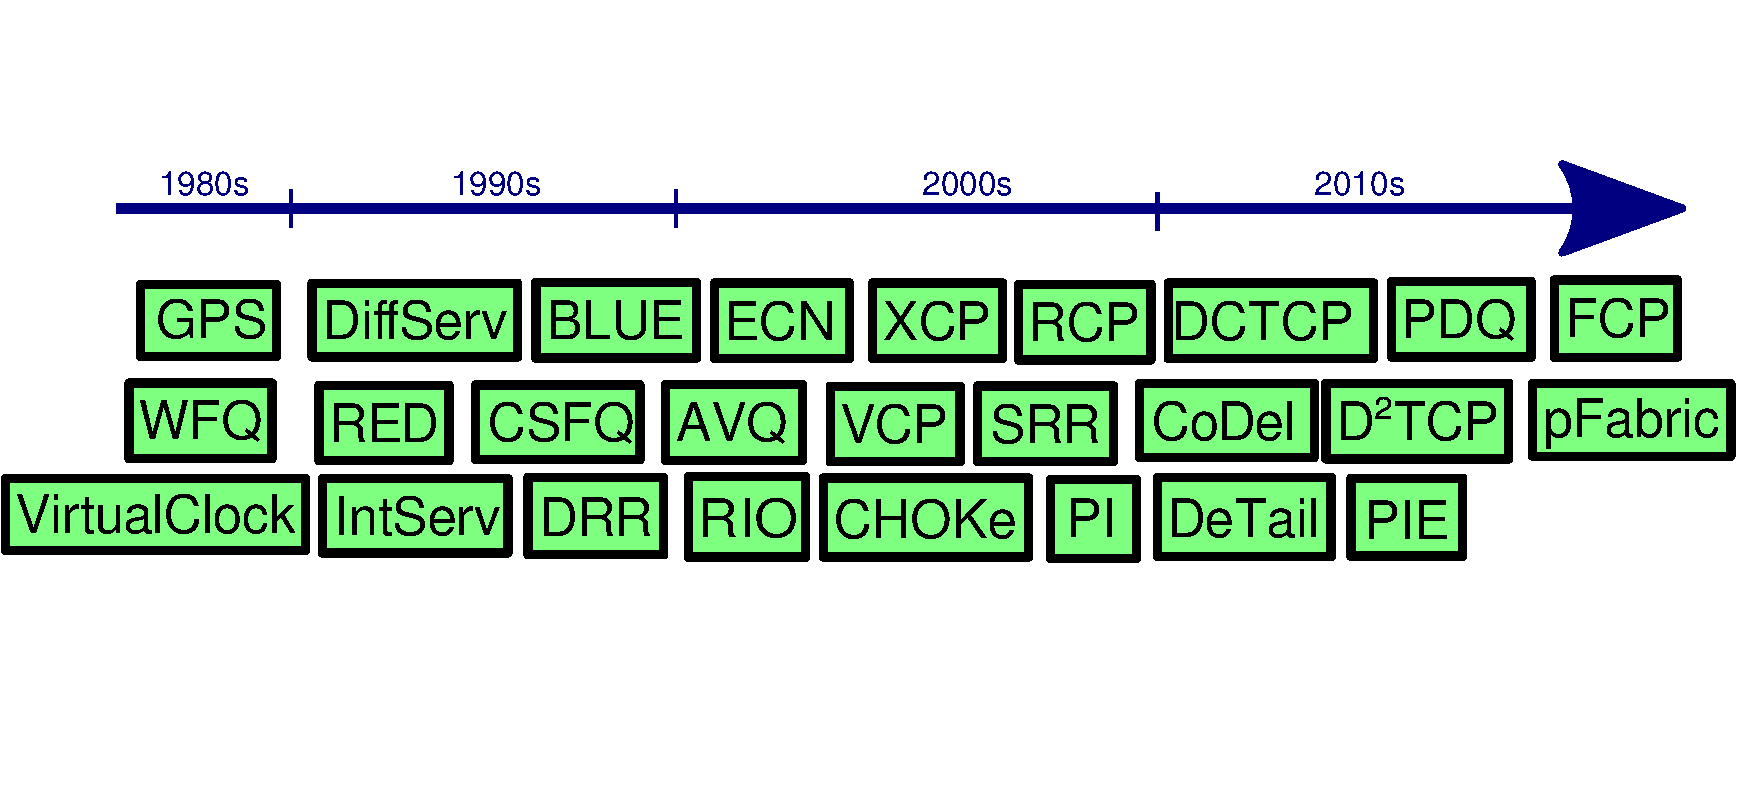
\includegraphics[width=1.0\textwidth]{march-1.pdf}}
\only<5>{\noindent \hspace{-.75 cm} 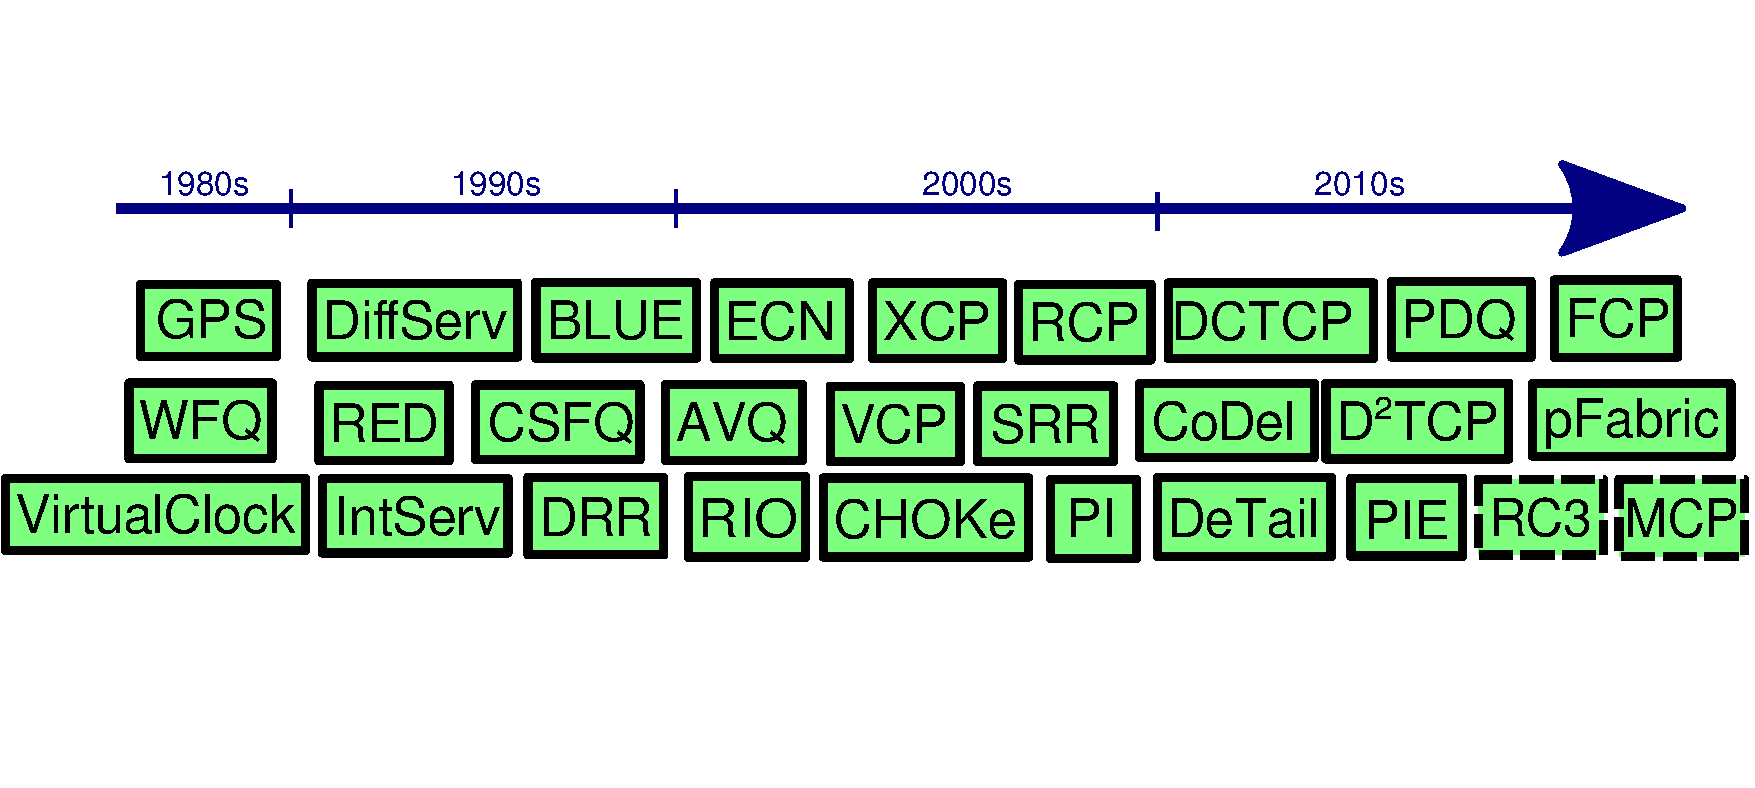
\includegraphics[width=1.0\textwidth]{march.pdf}}
\end{frame}


\begin{frame}[plain]
\frametitle{The Data Plane is continuously evolving}
\begin{itemize}
\item[]
\item Each scheme wins in its own evaluation.
\item[]
\item Some believe in a ``silver bullet'' knobless in-network method.
\end{itemize}
\end{frame}

\begin{frame}[plain]
\frametitle{We disagree: There is no silver bullet!}
\begin{itemize}
\item{Different applications care about different objectives.}
\item[]

\item{Applications use different transport protocols.}
\item[]

\item{Networks are heterogeneous.}

\end{itemize}
\end{frame}

\begin{frame}[plain]
\frametitle{Our work:}
\begin{itemize}
\item{Quantify non-universality of in-network methods.}
\item[]

\item{Extend SDN to the Data Plane to handle in-network diversity.}
\item[]

\end{itemize}
\end{frame}

%%
%%\begin{frame}[plain]
%%\frametitle{Early symptoms}
%%\begin{itemize}
%%\item{Hard to configure wired AQM for wireless links}
%%
%%\item[]
%%
%%\item{Several distinct point solutions for datacenters}
%%\begin{itemize}
%%\item DCTCP, HULL, D3, DeTail, PDQ, pFabric
%%\end{itemize}
%%
%%\item[]
%%
%%\item{No consensus on the ``right metric"}
%%\begin{itemize}
%%\item Minimizing missed deadlines
%%\item Flow Completion Time
%%\item Latency
%%\item Throughput
%%\item Tail Latency
%%\item \dots 
%%\end{itemize}
%%
%%\end{itemize}
%%\end{frame}
%%
\begin{frame}[plain]
\frametitle{Quantifying ``No Silver Bullet'': Network Configurations}
\begin{table}
\begin{tabular}{|p{0.34\linewidth}|p{0.65\linewidth}|}
\hline
{\bf \underline{Configuration}} & {\bf \underline{Description}} \\
{\bf CoDel+FCFS} & One shared FCFS queue with CoDel\\
& \\
%\hline
{\bf CoDel+FQ} & Per-flow fair queueing with CoDel on each queue\\ 
&\\
%\hline
{\bf Bufferbloat+FQ} & Per-flow fair queueing with deep buffers on
each queue\\ 
\hline
\end{tabular}
\end{table}
\end{frame}

\begin{frame}[plain]
\frametitle{Quantifying``No Silver Bullet'': Workloads and Objectives}

\begin{table}
\begin{tabular}{|p{0.22\linewidth}|p{0.33\linewidth}|p{0.38\linewidth}|}
\hline
{\bf \underline{Workload}} & {\bf \underline{Description}} & {\bf \underline{Objective}} \\
\textbf{\emph{Bulk}} & Long-running bulk transfer flow & Max. throughput \\
& &\\
\textbf{\emph{Web}} & Switched flow with ON and OFF periods &
Min. 99.9 \%ile flow completion time \\
& &\\
\textbf{\emph{Interactive}} & Long-running interactive flow & Max. $\frac{\mbox{throughput}}{\mbox{delay}}$ (power) \\ 
\hline
\end{tabular}
\end{table}
\end{frame}

\begin{frame}[plain]
\frametitle{Quantifying ``No Silver Bullet''}

\only<1>{ \noindent \begin{figure}[ht]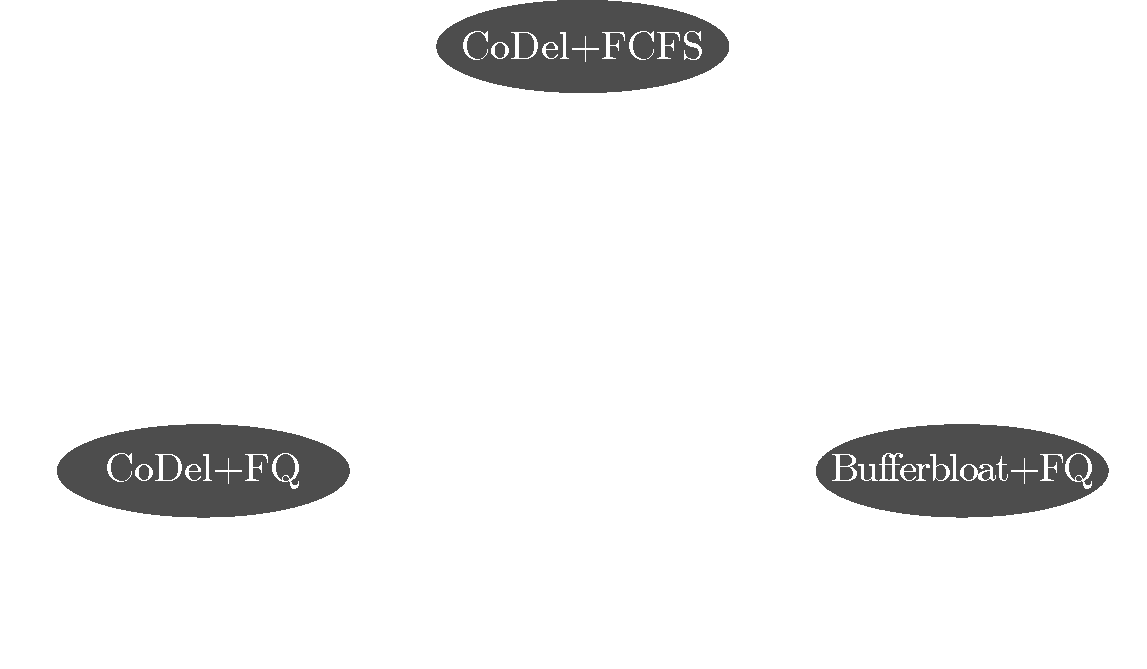
\includegraphics[width=\columnwidth]{fig-6.pdf}\end{figure}}

\only<2>{
  \begin{center}
  \begin{tabular}{| p{2.3cm} |p{3.5cm}| p{2.1cm}| }
  \hline
  Nwk config. & Avg. throughput, delay & Power\\
  \hline
  Bufferbloat+FQ  & 7.47 Mbps, 62165 ms & \cellcolor{red!20} 0.12 $Mbit/s^{2}$ \\
  \hline
  CoDel+FQ & 6.55 Mbps, 76.5 ms  & \cellcolor{green!20} 85.6 $Mbit/s^{2}$\\
  \hline
  \end{tabular}
  \end{center}
}
\only<3>{ \noindent \begin{figure}[ht]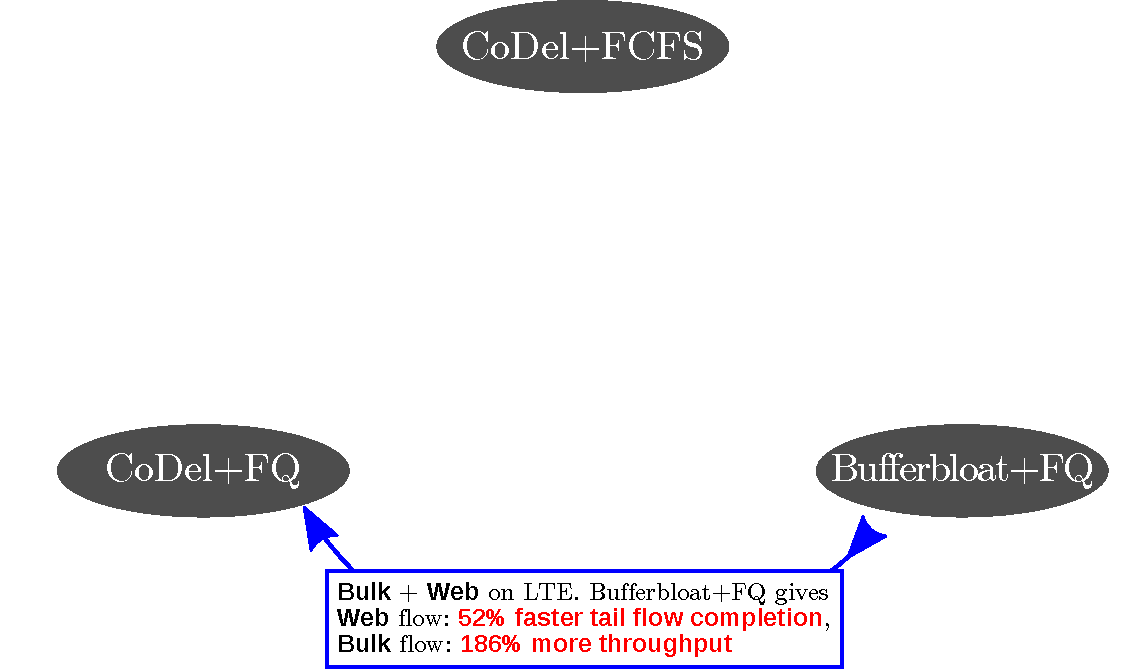
\includegraphics[width=\columnwidth]{fig-5.pdf}\end{figure}}

\only<4>{
  \begin{center}
  \begin{tabular}{| p{2.5cm} |p{2.5cm} | p{2cm} | }
  \hline
  Nwk config. & Bulk Throughput & Web Tail FCT\\
  \hline
  Bufferbloat+FQ & \cellcolor{green!20} 11.22 Mbps & \cellcolor{green!20} 20.94 secs \\
  \hline
  CoDel+FQ & \cellcolor{red!20} 3.92 Mbps & \cellcolor{red!20} 43.72 secs \\
  \hline
  \end{tabular}
  \end{center}
}
\only<5>{ \noindent \begin{figure}[ht]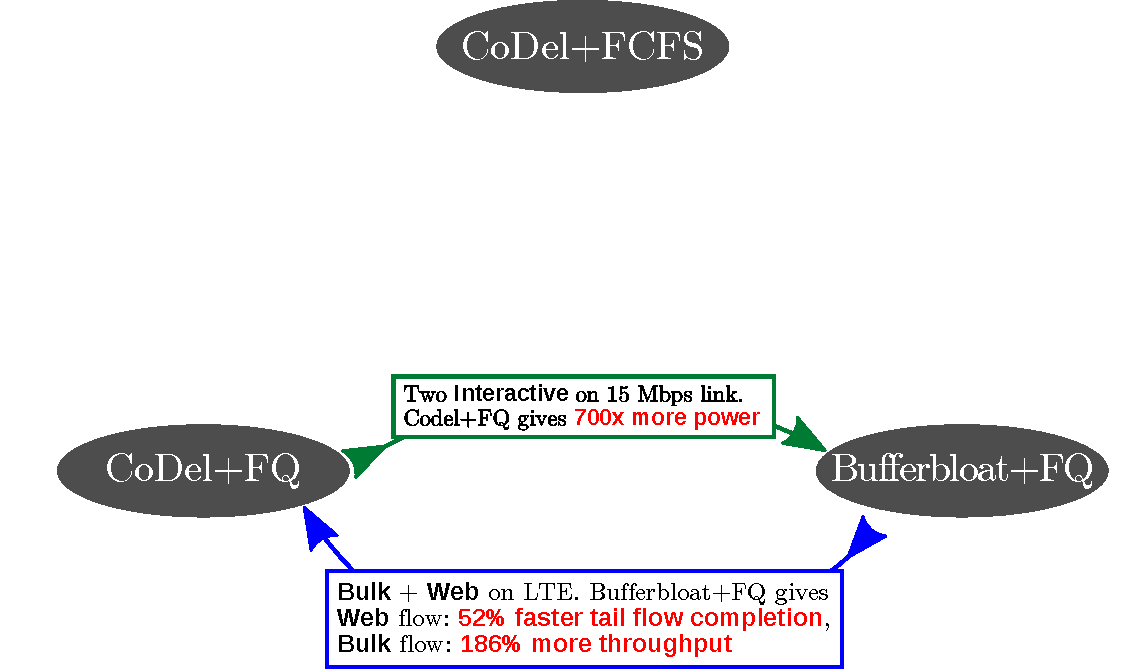
\includegraphics[width=\columnwidth]{fig-4.pdf}\end{figure}}

\only<6>{
  \begin{center}
  \begin{tabular}{| p{2cm} |p{4cm} | }
  \hline
  Nwk config. & Avg. throughput \\
  \hline
  CoDel+FCFS & \cellcolor{green!20} 2.00 Mbps \\
  \hline
  CoDel+FQ & \cellcolor{red!20} 1.90 Mbps \\
  \hline
  \end{tabular}
  \end{center}
}
\only<7>{ \noindent \begin{figure}[ht]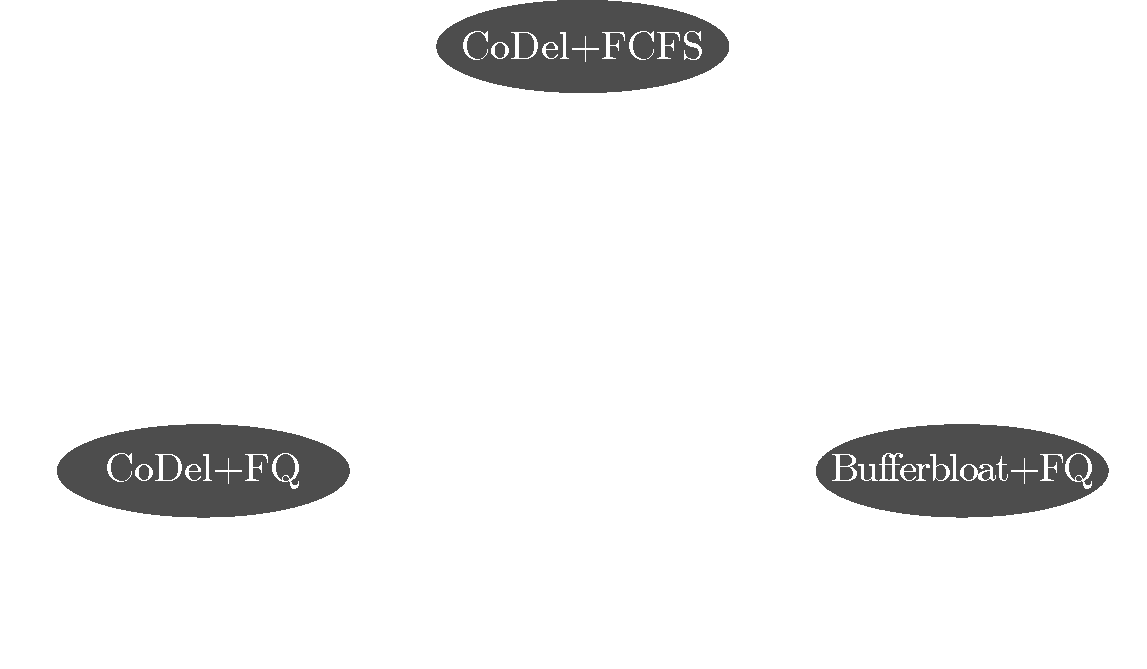
\includegraphics[width=\columnwidth]{fig-3.pdf}\end{figure}}

\only<8>{
  \begin{center}
  \begin{tabular}{| p{2cm} |p{2.5cm} | p{4cm} | }
  \hline
  Nwk config. & Bulk Throughput & Web Tail FCT  \\
  \hline
  CoDel+FCFS & 9.48 Mbps & \cellcolor{red!20} 22.25 secs \\
  \hline
  CoDel+FQ & 9.48 Mbps & \cellcolor{green!20} 18.71 secs \\
  \hline
  \end{tabular}
  \end{center}
}
\only<9>{ \noindent \begin{figure}[ht]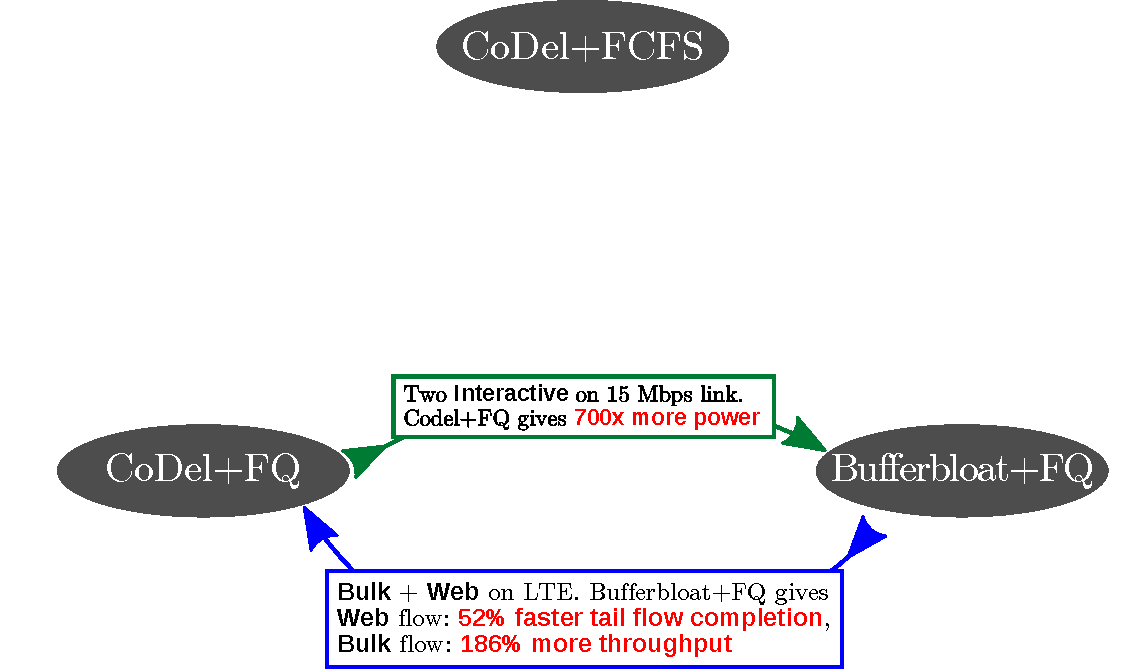
\includegraphics[width=\columnwidth]{fig-2.pdf}\end{figure}}

\only<10>{
  \begin{center}
  \begin{tabular}{| p{3.0cm} |p{3.0cm} |  }
  \hline
  Nwk config. & Bulk throughput  \\
  \hline
  Bufferbloat+FQ & \cellcolor{green!20} 11.96 Mbps \\
  \hline
  CoDel+FCFS & \cellcolor{red!20} 4.35 Mbps \\
  \hline
  \end{tabular}
  \end{center}
}
\only<11>{ \noindent \begin{figure}[ht]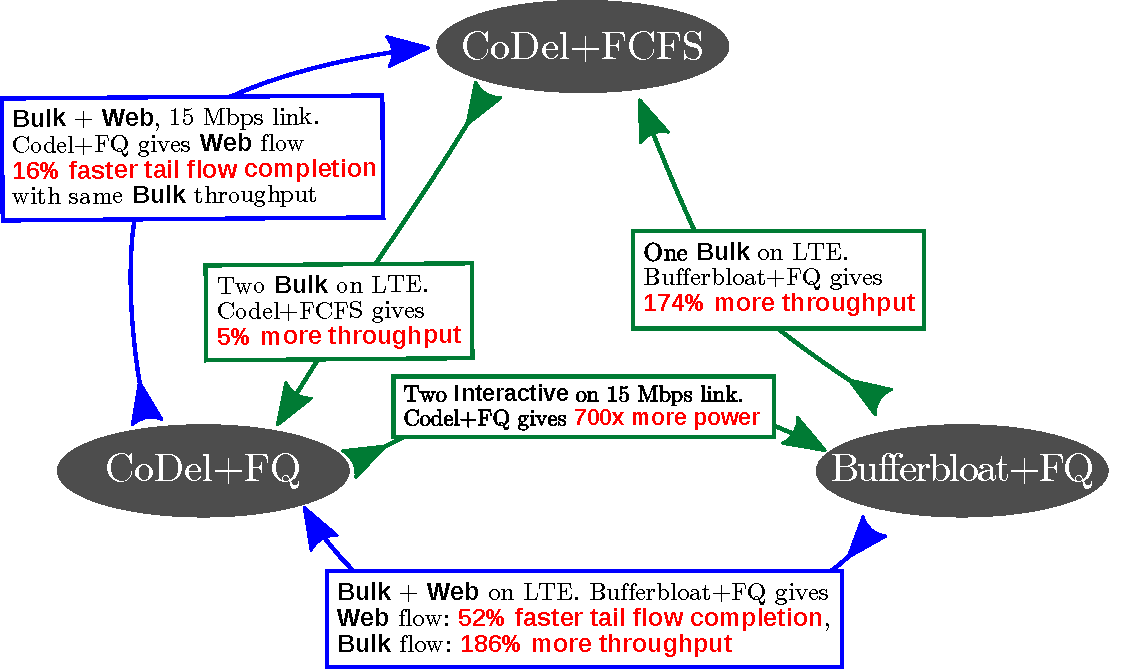
\includegraphics[width=\columnwidth]{fig-1.pdf}\end{figure}}

\only<12>{
  \begin{center}
  \begin{tabular}{| p{2.2cm} |p{4.2cm} |p{2.2cm}| }
  \hline
  Nwk config. & Interactive throughput, delay & Power\\
  \hline
  Bufferbloat+FQ & 11.96 Mbps, 46028~ms & \cellcolor{red!20} 0.26 $Mbit/s^{2}$\\
  \hline
  CoDel+FCFS & 4.35 Mbps, 83.2~ms & \cellcolor{green!20}52.28 $Mbit/s^{2}$ \\
  \hline
  \end{tabular}
  \end{center}
}
\only<13>{ \noindent \begin{figure}[ht]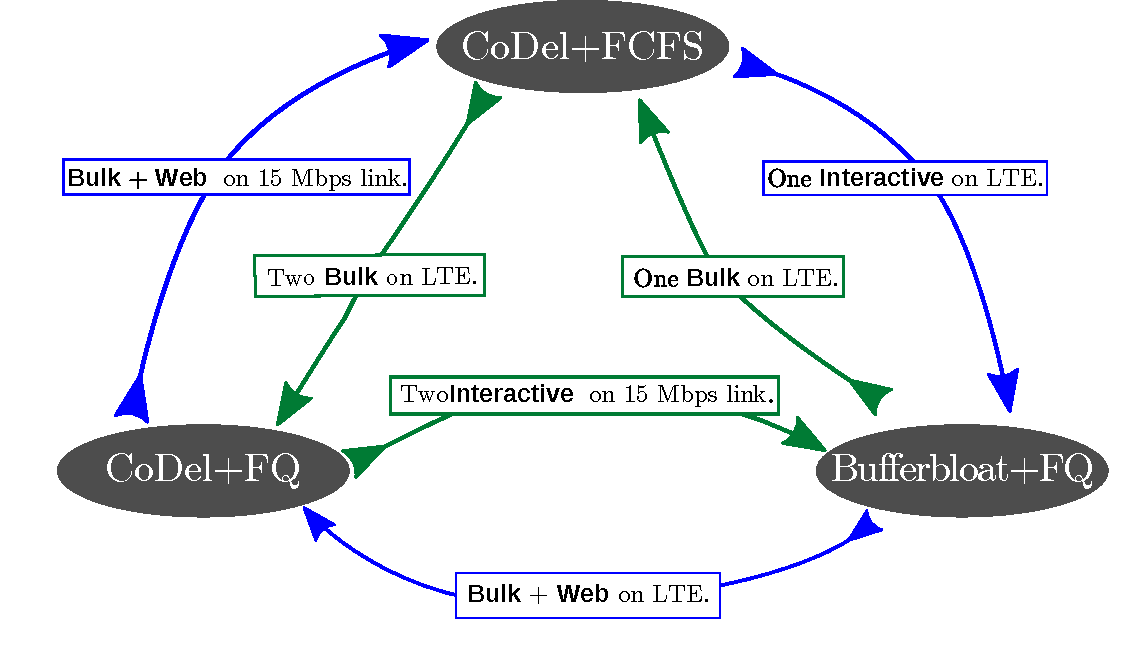
\includegraphics[width=\columnwidth]{fig.pdf}\end{figure}}


\end{frame}

\begin{frame}[plain]
\frametitle{Why is no single data plane configuration the best?}
\begin{itemize}
\item Bufferbloat on variable-rate links helps throughput!
      \begin{itemize}
      \item Variable-rate links have an inherent delay-throughput tradeoff
      \end{itemize} 

\item[] 

\item FCFS is preferable to Fair Queuing in some cases
      \begin{itemize}
      \item When equally aggressive flows compete, they don't need
        protection from each other
        \item Helps reduce tail packet delay
      \end{itemize}

\item[]

\item Fair Queuing is required in some cases
      \begin{itemize}      
      \item When competing flows aren't equally aggressive,
        isolation helps
      \end{itemize}
\end{itemize}
\end{frame}

\begin{frame}[plain]
\frametitle{So what should the network designer do?}
Architect a flexible data plane
\begin{itemize}
\item Programmable queue management and scheduling
\item Not just for selecting among pre-built choices, but to change
  behavior in the field
\item Because there is no silver bullet and innovation will continue!
\end{itemize}
\end{frame}

\begin{frame}[plain]
\frametitle{Controlled flexibility: Want performance, security}

% Mention previous talk here.
%(Or, why this isn't the same as ``active networks'')

\begin{itemize}
\item Provide interfaces only to the head and tail of queues
\item Operators specify only queue-management/scheduling logic
\item No access to packet payloads.
\end{itemize}
\end{frame}

\begin{frame}[plain]
\frametitle{Building such a data plane in four parts}
\begin{itemize}
\item Hardware gadgets
      \begin{itemize}
      \item Random number generators (RED, BLUE)
      \item Binary tree of comparators (pFabric, SRPT)
%      \item EWMA estimators (RED, AVQ, CSFQ)
      \end{itemize}

\item I/O interfaces
      \begin{itemize}
      \item Drop/mark head/tail of queue
      \item Interrupts for enqueue/dequeue
      \end{itemize}

\item State maintenance
      \begin{itemize}
      \item Per-flow (WFQ, DRR)
      \item Per-dst address (PF)
%      \item For fastest flows alone (AFD)
      \end{itemize}

\item A domain-specific instruction set
      \begin{itemize}
      \item Expresses control flow
      \item Implements new functions unavailable in hardware
      \end{itemize}
\end{itemize}
\end{frame}

\begin{frame}[plain]
\frametitle{Feasibility study: CoDel}
%\begin{center}
%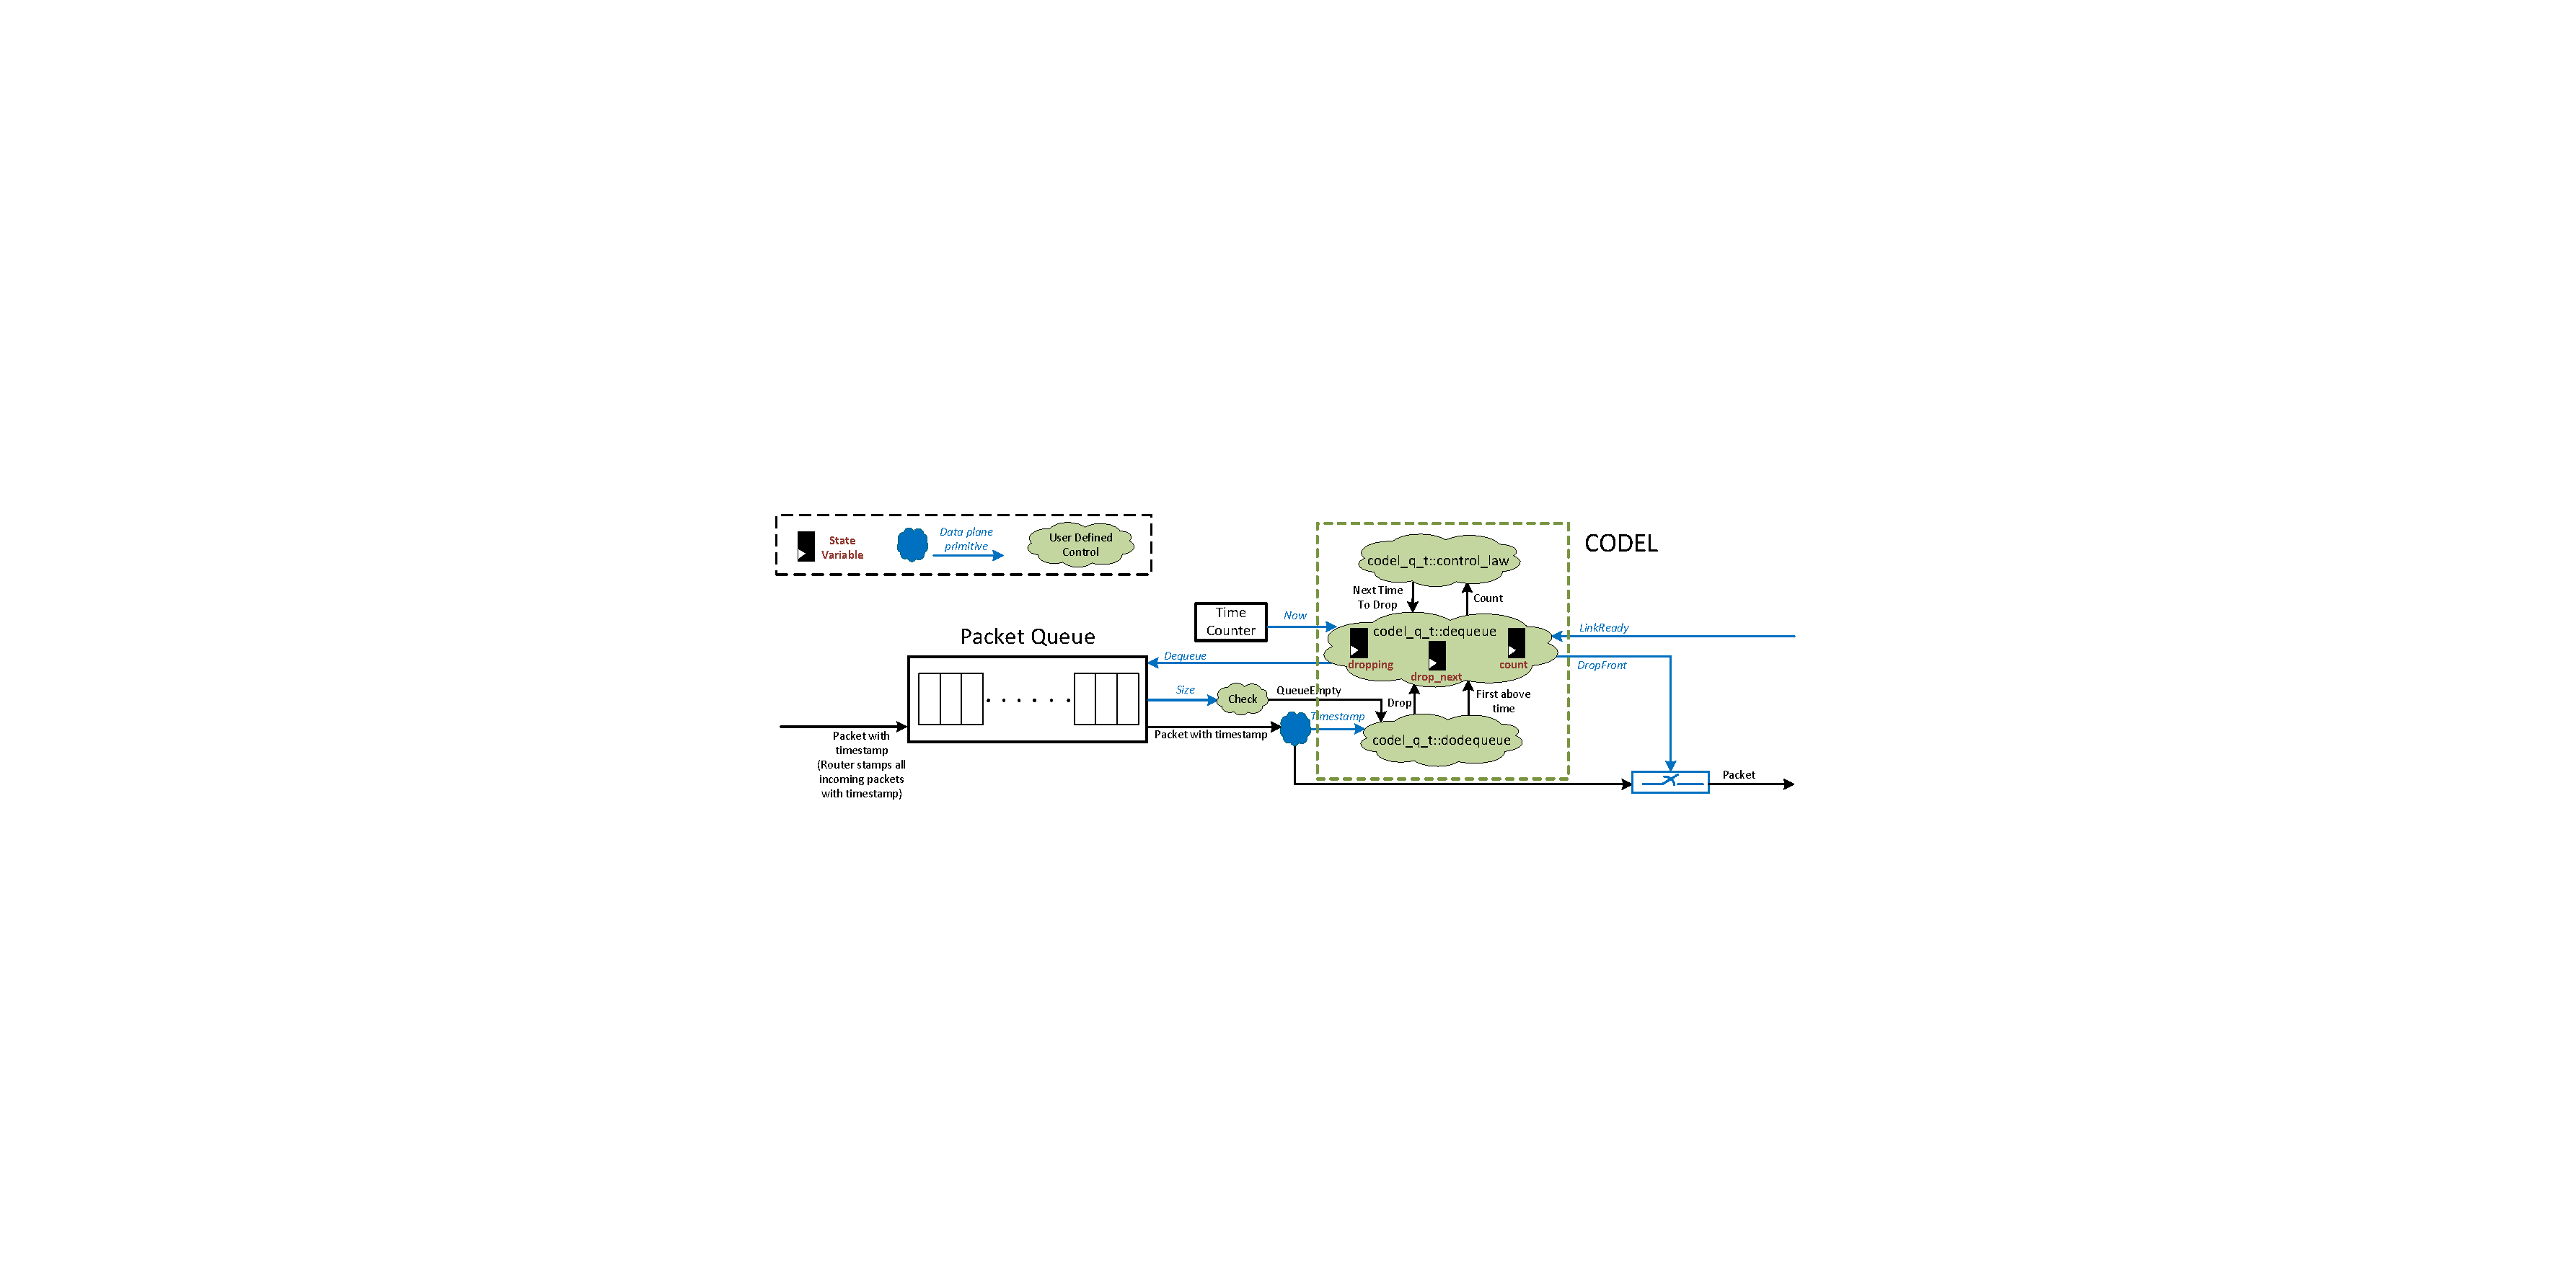
\includegraphics[width=\columnwidth]{codel.pdf}
%\end{center}
\begin{center}
Synthesis numbers on Xilinx Kintex-7: \\
\begin{tabular}{p{0.32 \columnwidth} p{0.32 \columnwidth} p{0.32 \columnwidth}}
\bf Resource & \bf Usage & \bf Fraction \\
\hline Slice logic & 1,256 & 1\% \\
Slice logic dist. & 1,975 & 2\% \\
IO/GTX ports & 27 & 2\% \\
DSP slices & 0 & 0\% \\
%TODO: Fix this.
Maximum speed & 12.9 $\times 10^6$ pkts/s \url{~ 10 gbps} \\
\end{tabular}
\end{center}
\begin{itemize}
\item Small fraction of the FPGA's resources.
\item Can be improved by pipelining or parallelizing.
\end{itemize}
\end{frame}

\begin{frame}[plain]
\frametitle{Limitations and Practical Considerations:}
\begin{itemize}
\item Cannot express several network functions that need payloads.
\item How do applications signal objectives to the network?
\item Feasibility at 10G on high port-density  switches.
\item Energy and Area overheads.
\end{itemize}
\end{frame}

\begin{frame}[plain]
\frametitle{Related Work:}
\begin{itemize}
\item Active Networking, e.g., ANTS
\item []
\item Software Routers, e.g., Click
\item []
\item Software-Defined Networking, e.g., OpenFlow
\end{itemize}
\end{frame}

\begin{frame}[plain]

\frametitle{Conclusion}
\begin{itemize}

\item There is no silver bullet to in-network resource control because
  of application and network diversity

\item[]
\item Algorithms will continue to evolve: the data plane should help

\item[]
\item Directions to reproduce results: \textcolor{DarkBlue}{http://web.mit.edu/anirudh/www/sdn-data-plane.html} 

\end{itemize}
\end{frame}


%% Backup slides 

\end{Large}
